\documentclass[12pt]{iptex}
% IDIOMA
% Se necessário, inserir línguas e indicar língua principal (main)
\usepackage[main=brazil,english]{babel}
\usepackage[italic]{mathastext}
\usepackage{siunitx}
\sisetup{
    group-separator={.},
    group-minimum-digits=3,
    output-decimal-marker={,}}

% Alterando nome do TOC (adicionar em outras línguas, se necessário)
\addto\captionsbrazil{%
	\renewcommand{\contentsname}{SUMÁRIO}
	\renewcommand{\refname}{REFERÊNCIAS}
}
\addto\captionsenglish{%
	\renewcommand{\contentsname}{CONTENTS}
	\renewcommand{\refname}{REFERENCES}
}
% BIBLIOGRAFIA
\usepackage[abnt-emphasize=bf,alf]{abntex2cite}
% Para bibliografia ABNT com números
%\usepackage[abnt-emphasize=bf,num]{abntex2cite}
%\citebrackets[]

% Para outros estilos o autor deve definir o \bibliographystyle dentro do documento

% Ajustes adicionais
\setlist[enumerate]{itemsep=3mm} % espaçamento enumerate
\setlist[itemize]{itemsep=3mm} % espaçamento itemize


% Início do documento
\begin{document}

% CAPA 
% Parâmetros
%\docNum{}
\tipo{BOLETIM SISMOLÓGICO}
%\cancelaDoc{Relatório Técnico nº 123 456-205} % Descomente para opção cancela e substitui
%\cliente{Instituto de Pesquisas Tecnológicas}{IPT}{Av. Professor Almeida Prado, 532}{55555-555}{São Paulo}{SP}
\data{2023}
\titulo{\textbf{RSIS - REDE SISMOLÓGICA XXXXXXXXXXXXXXXXXXXXXX} \\
\textbf{RESERVATÓRIOS BARRA GRANDE, SC/RS E CAMPOS NOVOS, SC} \\
\textbf{RELATÓRIO MENSAL DE ATIVIDADES}}
\unidade{Cidades Infraestruturas e Meio Ambiente}{CIMA}
\lab{Seção de Obras Civis - SOC}
\periodo{MES/ANO}{MES/ANO}


% Inserir capa
\capa
\pagestyle{timbrado}

% Inserir resumo
%\resumo[]{Teste}{}

%\tableofcontents

\vspace{0.5cm}

%\pagebreak
%\renewcommand{\thepage}{\arabic{page}}
%\setcounter{page}{1}

%\thispagestyle{geral}

\pagestyle{geral}


% Corpo
% Corpo do documento

% INFORMAÇÕES GERAIS 
\section{INFORMAÇÕES GERAIS}
A seguir são apresentadas informações gerais dos empreendimentos, do monitoramento sismológico, das condicionantes ambientais e do contrato de execução das atividades desta prestação de serviçoitado ou excluído. especializado na área de Sismologia.

\subsection{Características dos empreendimentos}
Os empreendimentos constituem-se dos Aproveitamentos Hidrelétricos de:
\begin{itemize}
    \item \textbf{Barra Grande}, situado no rio Pelotas, SC/RS, com o barramento na divisa dos municípios de Anita Garibaldi, SC (margem direita) e Pinhal da Serra, RS (margem esquerda). O reservatório ocupa parcialmente terras dos municípios de: Anita Garibaldi, Cerro Negro, Campo Belo do Sul, Capão Alto e Lages, no Estado de Santa Catarina e Pinhal da Serra, Esmeralda, Vacaria e Bom Jesus, no Estado do Rio Grande do Sul; e
    \item \textbf{Campos Novos}, situado no rio Canoas, SC, com o barramento na divisa dos municípios de Campos Novos, SC (margem direita) e Celso Ramos, SC (margem esquerda). O reservatório atinge áreas dos municípios de Abdon Batista, Anita Garibaldi, Campos Novos e Celso Ramos, no Estado de Santa Catarina.
\end{itemize}

A operação, manutenção e administração da UHE Barra Grande e da UHE Campos Novos são de responsabilidade da Energética Barra Grande S. A. e Campos Novos Energia S. A., respectivamente.

As características dos reservatórios, resumidamente, são:

\begin{table}[hb]
\centering
\begin{tabular}{|c|c|c|c|}
\hline
\multicolumn{2}{|c|}{\textbf{Características}} & \textbf{Barra Grande} & \textbf{Campos Novos} \\
\hline
\multicolumn{2}{|c|}{\textbf{Rios}} & Pelotas & Canoas \\
\hline
    \multirow{4}{*}{Coordenadas}
        & \multirow{2}{*}{Latitude}
            & 6.927.235,655 m N & 6.946.910,374 m N \\
            \cline{3-4}
            && 27,7667º S & 27,6010º S\\
            \cline{2-4}
        & \multirow{2}{*}{Longitude}
            & 481.136,036 m E & 467.699,707 m E \\
            \cline{3-4}
            && 51,2167º W & 51,3273º W \\
\hline
\multicolumn{2}{|c|}{Distância da Foz (km)} & 43 &  21 \\ \hline
\multicolumn{2}{|c|}{Área (km²)} & 93,4 &  34,6 \\ \hline
\multicolumn{2}{|c|}{Comprimento (km)} & 115 &  52 \\ \hline
\multicolumn{2}{|c|}{Volume (m³)} & 5.200 x 10^6 &  1.477 x 10^6 \\ \hline
\multicolumn{2}{|c|}{Cota da Lamina d'água (m) - montante} & 647 &  660 \\ \hline
\multicolumn{2}{|c|}{Cota da Lamina d'água (m) - jusante} & 461 &  474 \\ \hline
\multicolumn{2}{|c|}{Profundidade Máxima (m)} & 186 &  188 \\ \hline
    \multirow{2}{*}{Enchimento}
        & Início & 05.07.2005 & 10.10.2005/25.10.2005 \\
        \cline{2-4}
        & Término & 01.11.2005 & 26.11.2006/01.03.2007 (*) \\
        \hline
\multicolumn{2}{|c|}{Início da Operação} & 01.11.2005 & 03.02.2007 \\ \hline
\multicolumn{2}{|c|}{Potência Instalada (MW)} &  690 & 880 \\ \hline
\end{tabular}
\caption{(*) esvaziamento e enchimento do reservatório em decorrência de problema ocorrido no túnel II de desvio.}
\end{table}

\subsection{Informações sobre as condicionantes ambientais:}
As condicionantes da Licença de Operação referentes ao monitoramento sismológico são:
\begin{itemize}
    \item BAESA: Condicionante 2.1, item e, da Licença Ambiental de Operação no 447/2005, 2a Renovação, emitida em 26/03/2014 pelo Instituto Brasileiro do Meio Ambiente e dos Recursos Naturais Renováveis – IBAMA para a Usina Hidrelétrica Barra Grande, que determina a continuidade do Programa de Monitoramento Sismológico; e
    \item ENERCAN: Licença Ambiental de Operação no 9665/2014, emitida em 23.12.2014 pela Fundação do Meio Ambiente – FATMA do Estado de Santa Catarina para a Usina Hidrelétrica Campos Novos, que determina a execução do Monitoramento das Condições Sismológicas.
\end{itemize}

\subsection{O monitoramento sismológico}
O monitoramento sismológico visa detectar as atividades sísmicas, natural ou induzida, nas áreas de influência dos reservatórios dos Aproveitamentos Hidrelétricos de Barra Grande, SC/RS e de Campos Novos, SC, fornecendo diagnósticos sobre as características da sismicidade local e suas possíveis consequências, possibilitando tomar medidas mitigadoras, atendendo as necessidades previstas nos Programas Ambientais destes empreendimentos.
Os sismos estão agrupados nos Fatores do Meio Físico. Como Indicadores Ambientais serão avaliados: distribuição geográfica (localização dos epicentros), tamanho (magnitude e intensidade) e frequência de ocorrência (distribuição temporal). A análise conjunta dos resultados destes indicadores possibilitará qualificar (natural ou induzida, local ou regional) e quantificar (fraca/média/forte, intermitente/contínua etc.) a sismicidade fornecendo subsídios para outros programas, tais como: Gerenciamento de Riscos e Comunicação Social. Os resultados indicarão a necessidade ou não de uma redefinição do monitoramento sismológico deste estudo, com o intuito de se estudar adequadamente a atividade sísmica local.
O monitoramento local teve início em meados de fevereiro de 2004 com a instalação da Estação “vigilante” BCM2 para auscultar a sismicidade local na fase  prévia ao enchimento dos reservatórios e entre maio-dezembro de 2005 foram instaladas as outras 4 estações, compondo a RSBC – Rede Sismológica de Barra Grande e Campos Novos, para a auscultação nos períodos de enchimento e pós-enchimento dos reservatórios.

A seguir são apresentados os dados referentes à localização das estações da RSBC e as respectivas datas de instalação:
\begin{table}
% TABELA DA LOCALIZAÇÃO
\end{table}
\caption*{(**) em 20.01.2009 foi desativada e os equipamentos retornaram para a estação BC7}
\caption*{(*) em 26.01.2015 foi desativada a estação BC7.}
\caption*{A partir de janeiro de 2015 não estão sendo utilizados mais os dados da Estação BCM2.}

As estações sismológicas e os empreendimentos estão localizados em rochas basálticas toleíticas e riodacitos da bacia do Paraná.
O trabalho atual é uma continuação do monitoramento sismológico em execução na área, através da RSBC composta inicialmente de 5 estações digitais triaxiais de período curto, compreendendo a etapa de pAuditório István Jancsóós-enchimento dos citados reservatórios. Em função das características da sismicidade local, a partir de janeiro de 2015, a RSBC passou a funcionar com 3 estações (BC4, BC9 e BC12).
Cada estação sismológica é composta por registrador digital de 24 bits, sismômetro triaxial de período curto (fo = 1 Hz), ajuste do relógio/localização através de GPS (Global Position System), memórias flash para gravação dos dados e sistema de alimentação através de baterias estacionárias seladas e painéis solares.
No Anexo A, Figura 1, é apresentado o mapa da região de interesse do empreendimento com a localização das estações e eventos no entorno (caso existam) para o período abrangido pelo presente boletim sísmico.
Este estudo também contribuirá com informações sobre a ocorrência de sismos nos Estados de Santa Catarina, do Rio Grande do Sul e regiões vizinhas, contribuindo com dados, melhorando o conhecimento da sismicidade brasileira.
Em função das características operacionais das estações sismológicas e/ou dos eventos sísmicos que venham a ocorrer, serão obtidas também informações sobre atividade sísmica regional e mundial.
No atual estudo, a continuidade do monitoramento sismológico consiste das atividades que basicamente englobam: coleta e envio dos dados, a sua interpretação e a emissão de boletins sísmicos mensais e de relatórios técnicos semestrais, contendo os resultados da análise, considerações sobre a sismicidade e recomendações.

\subsection{O contrato de execução do serviço:}

A Instituição responsável pelo monitoramento sismológico:
Instituto de Pesquisas Tecnológicas do Estado de São Paulo S. A. - IPT
Av. Prof. Almeida Prado, 532 – CEP 05508-901
Cidade Universitária – Butantã – São Paulo – SP
CNPJ: 60.633.674/0001-55
IE: 105.933.432.110
Com relação ao CTF/CR - Cadastro Técnico Federal/Certificado de Regularidade tem-se que:
Responsável
Registro
Validade
Chave de Autenticação
Pessoa
IPT
676518
19/10/2023
Z7FX6S4TNR1QGXE8
Jurídica


E as ARTs – Anotação de Responsabilidade Técnica (CREA- SP):
Empresa
Nº
Emissão
Validade
BAESA
28027230230714974
30.05.2023
30.11.2024
ENERCAN
28027230230711325
30.05.2023
30.11.2024
OBS.: cópias dos CTFs e das ARTs encontram-se apresentadas no final deste Relatório Mensal de Atividade, no Anexo B.




\clearpage
% ÚLTIMOS RELATÓRIOS TÉCNICOS
\section{ÚLTIMO RELATÓRIO TÉCNICO}
\label{section:ultimo_relatorio}
\textbf{Relatório Barra Grande}:

\begin{itemize}
\item Relatório IPT no 168 887-205 – “Análise dos registros obtidos entre novembro de 2021 e outubro de 2022 na rede Sismológica de Barra Grande e Campos Novos–RSBC, referente ao reservatório de Barra Grande, SC/RS.”
\end{itemize}

\textbf{Relatório Campos Novos}:
\begin{itemize}
    \item Relatório IPT no 168 888-205 – “Análise dos registros obtidos entre novembro de 2021 e outubro de 2022 na rede Sismológica de Barra Grande e Campos Novos–RSBC, referente ao reservatório de Campos Novos, SC.”
\end{itemize}


% ATIVIDADES REALIZADAS 
\section{ATIVIDADES DESENVOLVIDAS}

\begin{itemize}
    \item Recebimento dos dados das coletas:
        \begin{itemize}
            \item BC4 – 14.04.2023 a 08.05.2023 e 08.05.2023 a 05.06.2023;
            \item BC9 – 11.04.2023 a 10.05.2023 e 10.05.2023 a 13.06.2023; 
            \item BC12 – 11.04.2023 a 10.05.2023 e 10.05.2023 a 13.06.2023;
        \end{itemize}
    \item Análise da completeza dos dados no período; e
    \item Análise preliminar dos dados das coletas supracitadas para o mês de maio.2023.
\end{itemize}


% RESULTADOS 
\section{RESULTADOS}
\par{Durante o mês de maio.2023 não foram detectados sismos induzidos na vizinhança dos reservatórios de Barra Grande e Campos Novos. Não há relatos de nenhum sismo que tenha sido sentido pela população local.}
\par{Foi detectado 1 desmonte em obras/pedreiras no período, com magnitude 1.7 MLv em 2023-05-19 16:06:00 (UTC), distante da região dos reservatórios.}
\par{Não foram detectados sismos naturais locais/regionais ou telessismos (sismos com epicentros distantes) no território brasileiro durante o período.}
\par{Na Tabela \ref{tab:tabela_baesa} encontram-se descritas as características e os parâmetros epicentrais do evento detectado pela RSBC no mês de maio.2023. As estações BC4, BC9 e BC12 operaram normalmente no período.}
\par{O funcionamento das estações foi satisfatório para o período, embora se haja constatado problema com a componente de registro Norte-Sul da estação BC9. A completeza dos dados para o período é mostrada na Figura 2, Anexo A.}

\begin{center}
\label{tab:tabela_baesa}
\scriptsize
\setlength{\arrayrulewidth}{0.05pt}
\begin{longtable}{ccccS[table-format=6.0]S[table-format=7.0]ccc}
\captionsetup{justification=justified,singlelinecheck=false}
\caption{Listagem de eventos detectados e categorizados durante o período de interesse.\\ A coluna \textit{Cat} representaria a categoria na qual o evento foi classificado sendo \textit{Q}=Detonação/Desmontes, \textit{E}=Sismo Regional e \textit{I}=Sismo induzido e \textit{N}=Não-localizável. O valor da energia para os sismos foi obtido a partir da magnitude através da relação proposta por Richter (1958).}\\
%%%%%%%%%%%%%%%%%%%%%%%%%%%%%%%%%%%%%%%%%%%%%%%%%%%%%%%
\hline \\[-4ex]
\hline \\[-5ex]
\multicolumn{1}{c}{ID} &
\multicolumn{1}{c}{Hora de Origem (UTC)} &
\multicolumn{1}{c}{Longitude} &
\multicolumn{1}{c}{Latitude} &
\multicolumn{1}{c}{UTM X} &
\multicolumn{1}{c}{UTM Y} &
\multicolumn{1}{c}{MLv} &
\multicolumn{1}{c}{Energia} &
\multicolumn{1}{c}{Cat} \\


\\[-5.0ex] \hline
\\[-5.0ex]

\multicolumn{1}{c}{\textit{{}}} & 
\multicolumn{1}{c}{\textit{{}}} & 
\multicolumn{1}{c}{\textit{(\textdegree\hspace{0.25em})}} & 
\multicolumn{1}{c}{\textit{(\textdegree\hspace{0.25em})}} & 
\multicolumn{1}{c}{\textit{{(m)}}} & 
\multicolumn{1}{c}{\textit{{(m)}}} & 
\multicolumn{1}{c}{\textit{{}}} & 
\multicolumn{1}{c}{\textit{{(J)}}} & 
\multicolumn{1}{c}{\textit{{}}} \\ 

\\[-5.0ex] \hline
\\[-4.0ex]
\endfirsthead


%%%%%%%%%%%%%%%%%%%%%%%%%%%%%%%%%%%%%%%%%%%%%%%%%%%%%%%
\hline \\[-4ex]
\hline \\[-5ex]
\multicolumn{1}{c}{ID} &
\multicolumn{1}{c}{Hora de Origem (UTC)} &
\multicolumn{1}{c}{Longitude} &
\multicolumn{1}{c}{Latitude} &
\multicolumn{1}{c}{UTM X} &
\multicolumn{1}{c}{UTM Y} &
\multicolumn{1}{c}{MLv} &
\multicolumn{1}{c}{Energia} &
\multicolumn{1}{c}{Cat} \\


\\[-5.0ex] \hline
\\[-5.0ex]

\multicolumn{1}{c}{\textit{{}}} & 
\multicolumn{1}{c}{\textit{{}}} & 
\multicolumn{1}{c}{\textit{(\textdegree\hspace{0.25em})}} & 
\multicolumn{1}{c}{\textit{(\textdegree\hspace{0.25em})}} & 
\multicolumn{1}{c}{\textit{{(m)}}} & 
\multicolumn{1}{c}{\textit{{(m)}}} & 
\multicolumn{1}{c}{\textit{{}}} & 
\multicolumn{1}{c}{\textit{{(J)}}} & 
\multicolumn{1}{c}{\textit{{}}} \\

\\[-5.0ex] \hline
\\[-4.0ex]
\endhead
\hline
\caption*{Fonte: IPT.}

\endlastfoot
%%%%%%%%%%%%%%%%%%%%%%%%%%%%%%%%%%%%%%%%%%%%%%%%%%%%%%%
MC\_20230830\_183917 & 2023-08-30T18:39:17 & -49,7253 & -27,1233 & 626336 & 6999266 & 1,3 & \num[round-precision=3,round-mode=figures,scientific-notation=true]{192765} & Q \\
MC\_20230824\_152934 & 2023-08-24T15:29:34 & -49,8028 & -27,1492 & 618629 & 6996476 & 1,5 & \num[round-precision=3,round-mode=figures,scientific-notation=true]{489398} & Q \\
MC\_20230822\_153204 & 2023-08-22T15:32:04 & -49,8803 & -26,8769 & 611218 & 7026705 & 1,7 & \num[round-precision=3,round-mode=figures,scientific-notation=true]{1.40658e+06} & Q \\
MC\_20230818\_154804 & 2023-08-18T15:48:04 & -49,7430 & -27,2696 & 624424 & 6983077 & 1,5 & \num[round-precision=3,round-mode=figures,scientific-notation=true]{665616} & Q \\
MC\_20230815\_192736 & 2023-08-15T19:27:36 & -49,8482 & -27,9594 & 613296 & 6906757 & 1,2 & \num[round-precision=3,round-mode=figures,scientific-notation=true]{150265} & Q \\
MC\_20230815\_191541 & 2023-08-15T19:15:41 & -50,5589 & -27,8340 & 543432 & 6921103 & 1,5 & \num[round-precision=3,round-mode=figures,scientific-notation=true]{620197} & E \\
MC\_20230815\_152902 & 2023-08-15T15:29:02 & -49,7932 & -27,1799 & 619550 & 6993060 & 1,8 & \num[round-precision=3,round-mode=figures,scientific-notation=true]{2.4461e+06} & Q \\
MC\_20230814\_152826 & 2023-08-14T15:28:26 & -49,8405 & -27,0239 & 615021 & 7010383 & 1,1 & \num[round-precision=3,round-mode=figures,scientific-notation=true]{86207.8} & Q \\
MC\_20230809\_105318 & 2023-08-09T10:53:18 & -51,3027 & -27,6952 & 470149 & 6936521 & -0,9 & \num[round-precision=3,round-mode=figures,scientific-notation=true]{14.7546} & I \\
MC\_20230808\_180349 & 2023-08-08T18:03:49 & -51,6466 & -27,3376 & 436040 & 6976001 & 0,5 & \num[round-precision=3,round-mode=figures,scientific-notation=true]{7229.98} & Q \\
MC\_20230808\_124749 & 2023-08-08T12:47:49 & -51,9186 & -28,7091 & 410272 & 6823898 & 1,3 & \num[round-precision=3,round-mode=figures,scientific-notation=true]{201872} & Q \\
MC\_20230803\_180211 & 2023-08-03T18:02:11 & -52,0653 & -28,7992 & 396036 & 6813799 & 1,5 & \num[round-precision=3,round-mode=figures,scientific-notation=true]{541480} & Q \\
MC\_20230802\_202746 & 2023-08-02T20:27:46 & -50,5841 & -27,9327 & 540915 & 6910184 & 1,4 & \num[round-precision=3,round-mode=figures,scientific-notation=true]{335748} & Q \\
MC\_20230802\_154527 & 2023-08-02T15:45:27 & -51,2518 & -27,4233 & 475109 & 6966653 & 0,8 & \num[round-precision=3,round-mode=figures,scientific-notation=true]{24333.2} & Q \\
MC\_20230801\_182340 & 2023-08-01T18:23:40 & -49,6500 & -27,1915 & 633720 & 6991634 & 1,2 & \num[round-precision=3,round-mode=figures,scientific-notation=true]{142694} & Q \\
MC\_20230801\_181715 & 2023-08-01T18:17:15 & -49,6761 & -27,6211 & 630624 & 6944073 & 1,9 & \num[round-precision=3,round-mode=figures,scientific-notation=true]{3.50567e+06} & Q \\
\end{longtable}
\end{center}
\clearpage




% CONSIDERAÇÕES 
\section{CONSIDERAÇÕES}
\par{A auscultação sismológica pode ser mantida, em função das características da sismicidade registrada na área de influência destes empreendimentos. O monitoramento sísmico também proporciona grande ajuda no entendimento da sismicidade Brasileira, especialmente nos estados do RS e SC.}\\
\par{Observa-se a presença de ruído sísmico nas estações RSBC durante horário comercial.  Na estação BC4 este ruído é constante em duas das três componentes, enquanto nas estações BC9 e BC12 ocorre de forma intermitente. As causas foram averiguadas em campo, e se trata de ruído de origem antrópica. Ressalta-se que a presença deste ruído não compromete de maneira significativa o monitoramento dos reservatórios, dado as estações operando em redundância na localidade.}\\

\assinaturaLucas


\begin{table}[b]
  \begin{adjustwidth}{0pt}{-9cm} % Ajusta a margem direita em -3cm
  \centering
  \setlength{\arrayrulewidth}{0.9pt} % Espessura das linhas verticais
  \begin{tabular}{|c|}
    \hline
    Cidades, Infraestrutura e Meio Ambiente \\
    \hline
    Seção de Obras Civis \\
    \hline \\[1.0pt]
    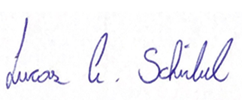
\includegraphics{./figuras/assinatura.png} \\[5.0pt]
    \hline \\[-25.0pt]
    Físico Me. Lucas Alexandre Schirbel \\[-7.0pt]
    Pesquisador \\[-7.0pt]
    RE: 117113 \\[0.0pt]
    \hline
  \end{tabular}
  \end{adjustwidth}
\end{table}

\clearpage
% ANEXOS
\clearpage
\vspace*{\fill}
\begin{center}
    \section*{ANEXO A}
\end{center}
\vspace*{\fill}
\clearpage
\newpage


\begin{figure}[ht!]
    \centering
	\captionsetup{justification=justified, singlelinecheck=false, width=1\textwidth}
    \caption{Mapa da região de interesse no entorno do empreendimento, mostrando as principais cidades, rodovias e rios, com a localização das pedreiras, estações \textbf{BCM2} e \textbf{MC9}, e eventos próximos ao empreendimento detectados no período de interesse.}
    \begin{mdframed}[
        linecolor=black,
        linewidth=1pt,
        roundcorner=10pt,
    ]
    \begin{center}
    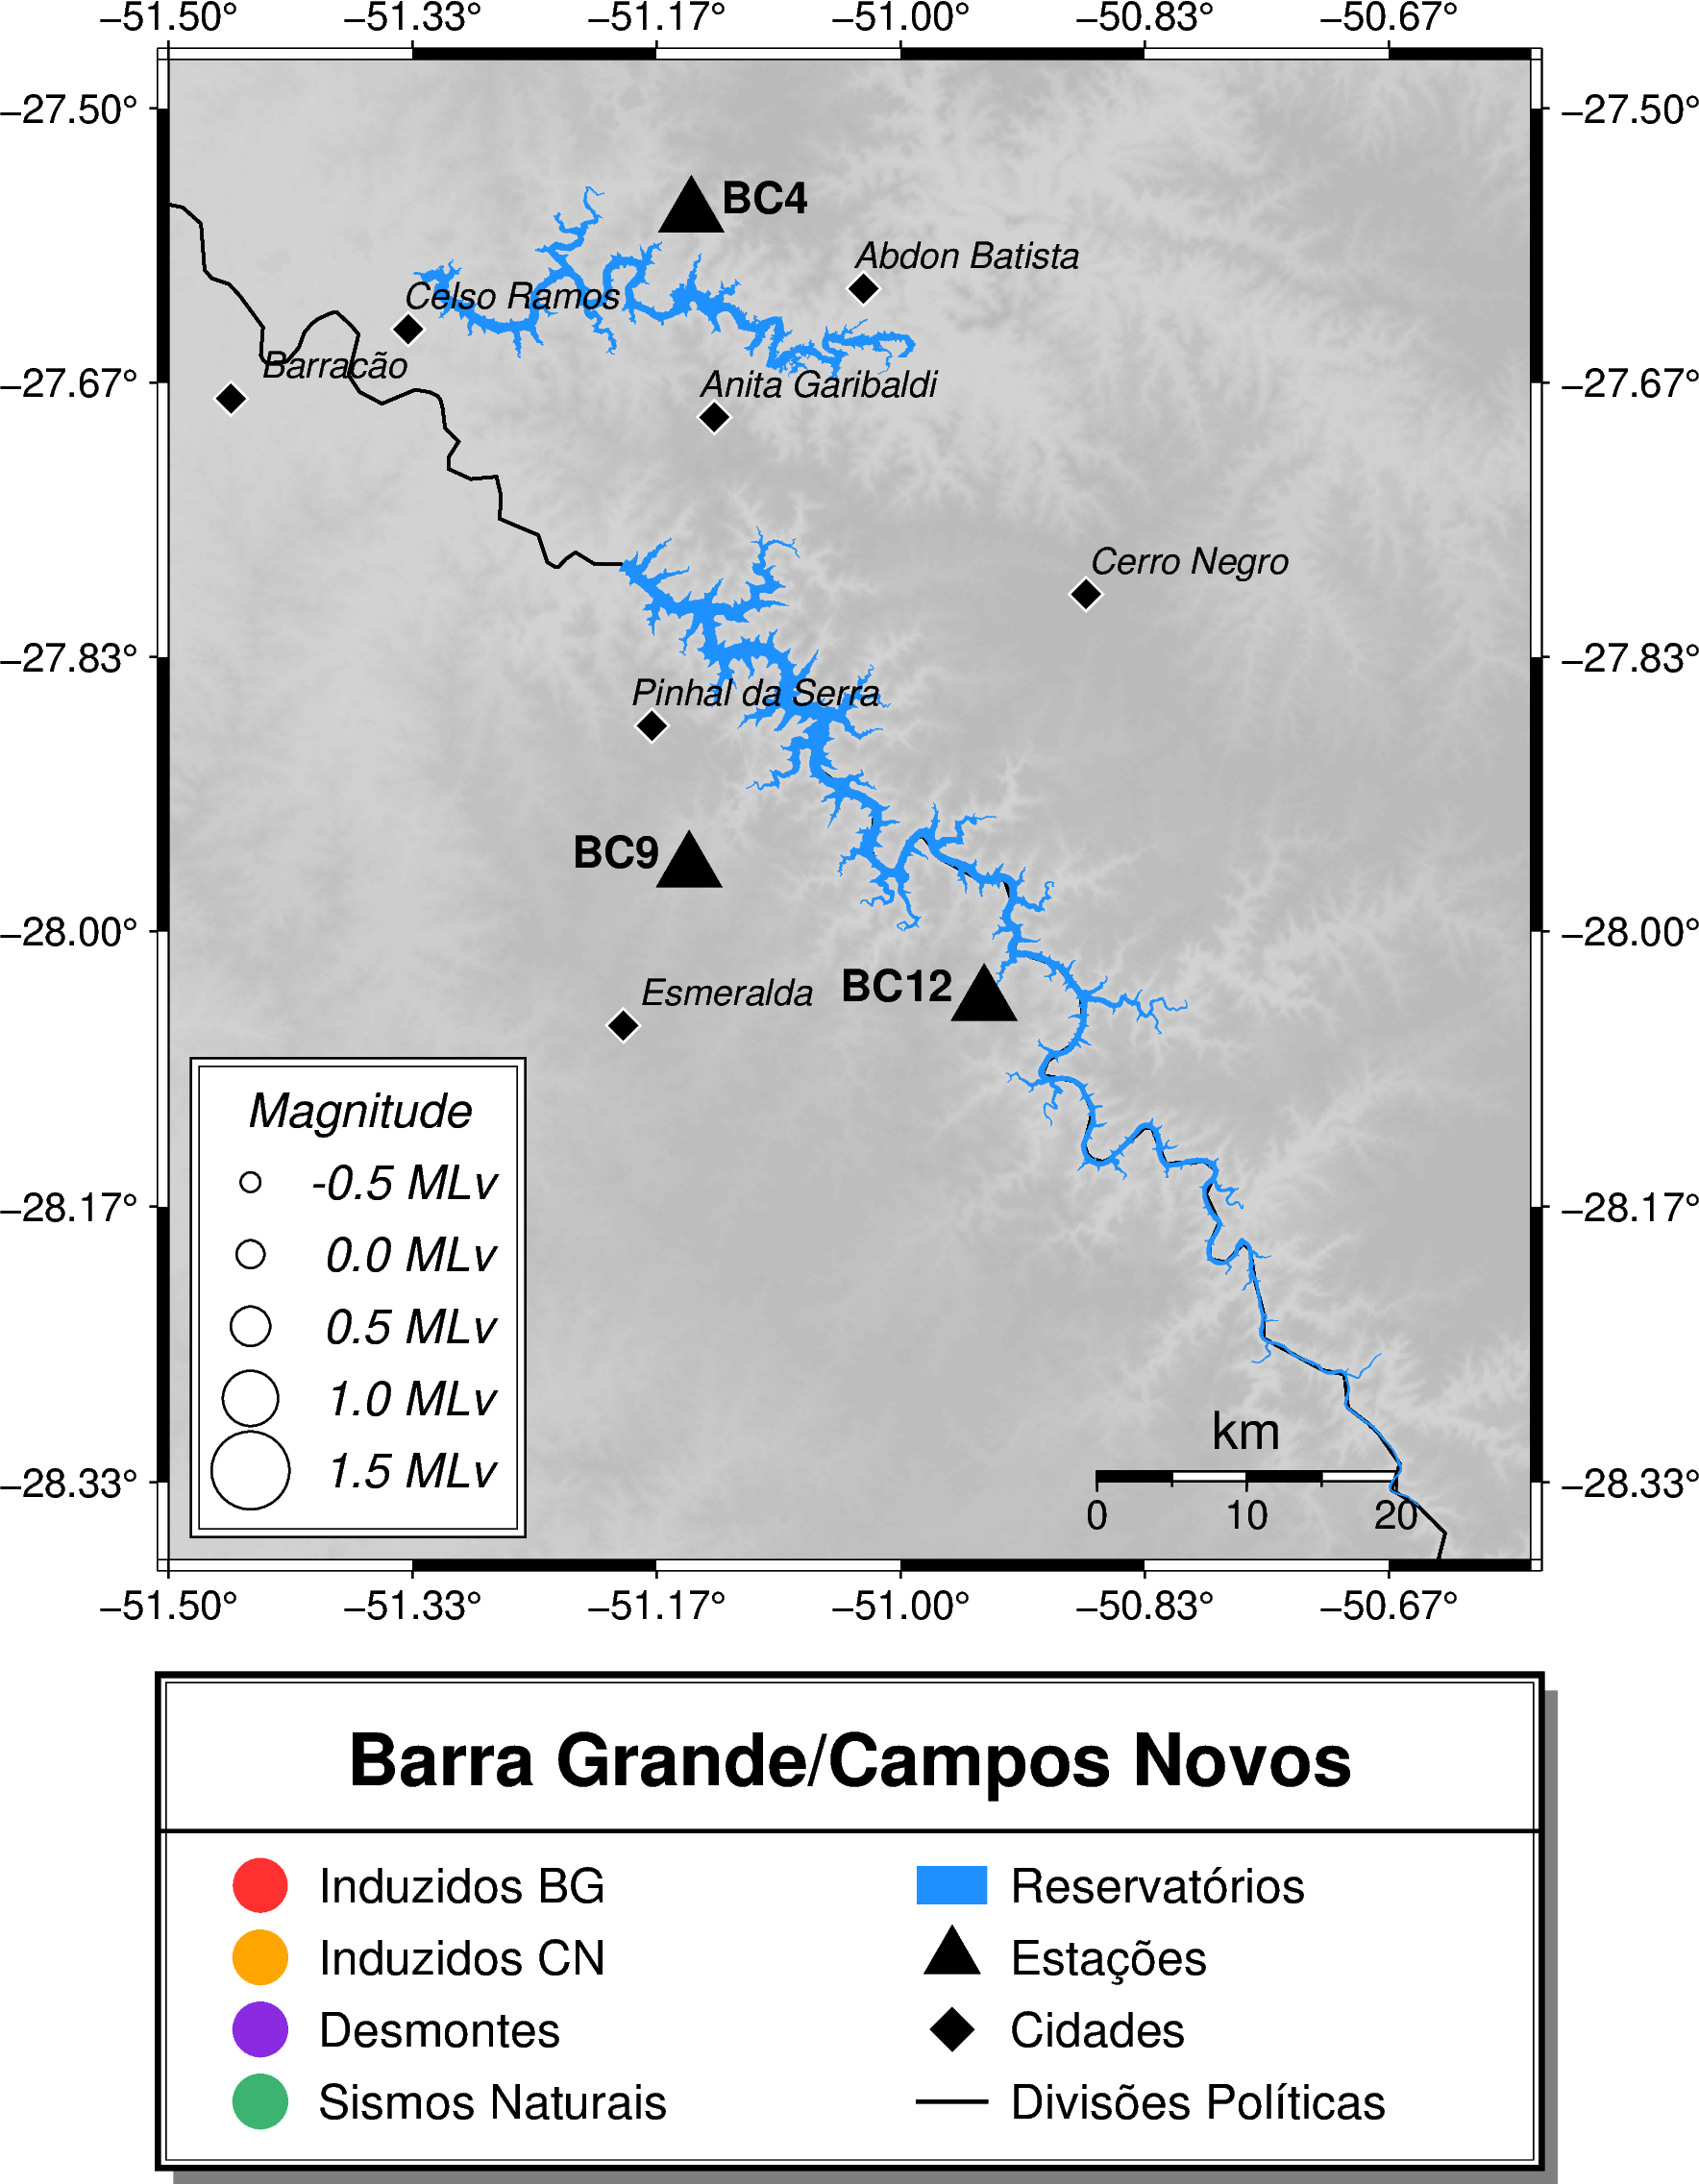
\includegraphics[width=0.8\textwidth]{../boletim/baesa/figuras/mapa_baesa.png}
    \end{center}
    \end{mdframed}
    \caption*{Fonte: IPT}
\end{figure}

\clearpage

\begin{figure}[ht!]
    \centering
	\captionsetup{justification=justified, singlelinecheck=false, width=1\textwidth}
    \caption{Gráficos de completeza dos dados para as estações BC4, BC9 e BC12 durante o período do mês de maio.2023. O registro de todas as estações foi satisfatório durante o período. Para a estação BC4, os últimos dois dias não foram incluídos por problemas na transmissão dos dados para o IPT, entretanto, serão analisados e incluídos no relatório anual. }
    \begin{mdframed}[
        linecolor=black,
        linewidth=1pt,
        roundcorner=10pt,
    ]
    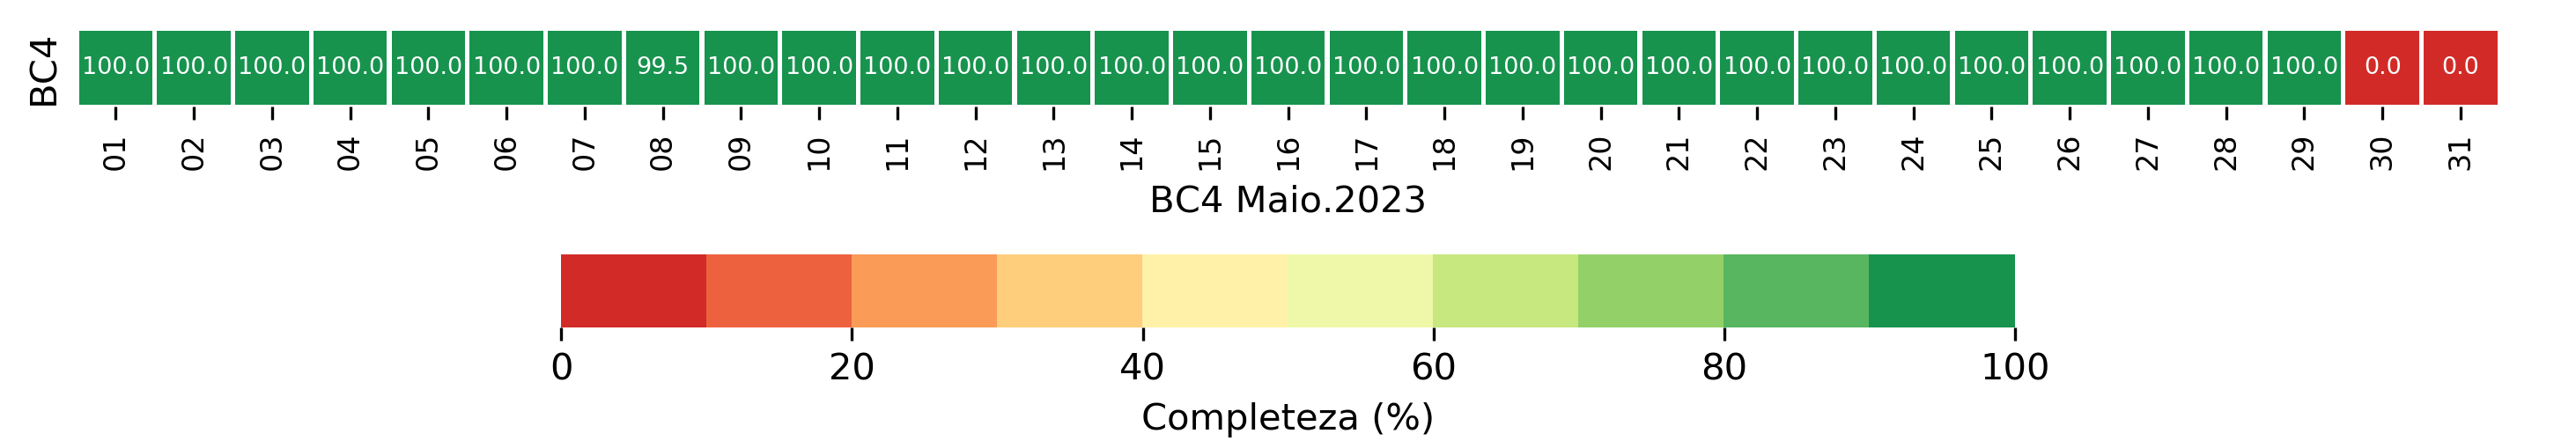
\includegraphics[width=1.0\textwidth]{./boletim/baesa/figuras/bc4_completude.png}
    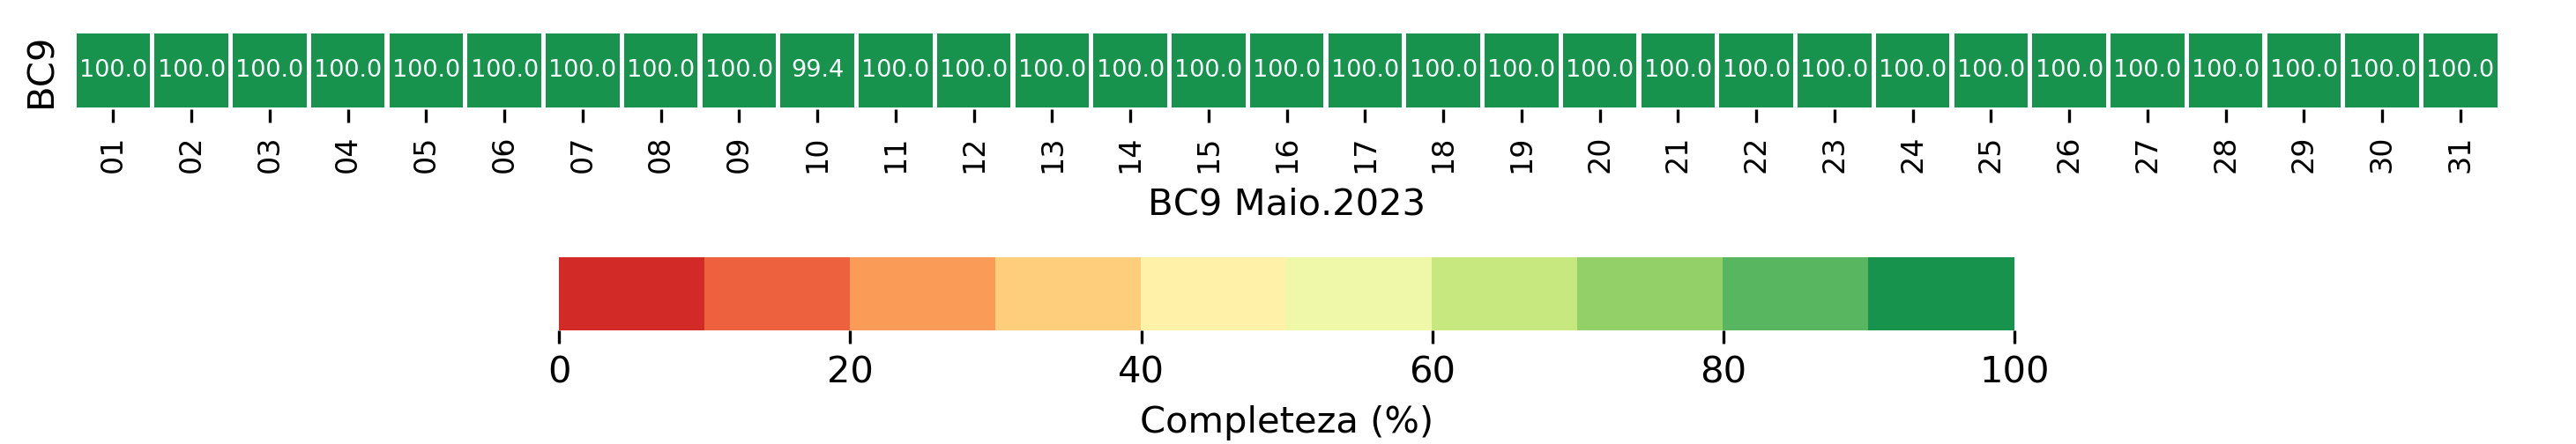
\includegraphics[width=1.0\textwidth]{./boletim/baesa/figuras/bc9_completude.png}
    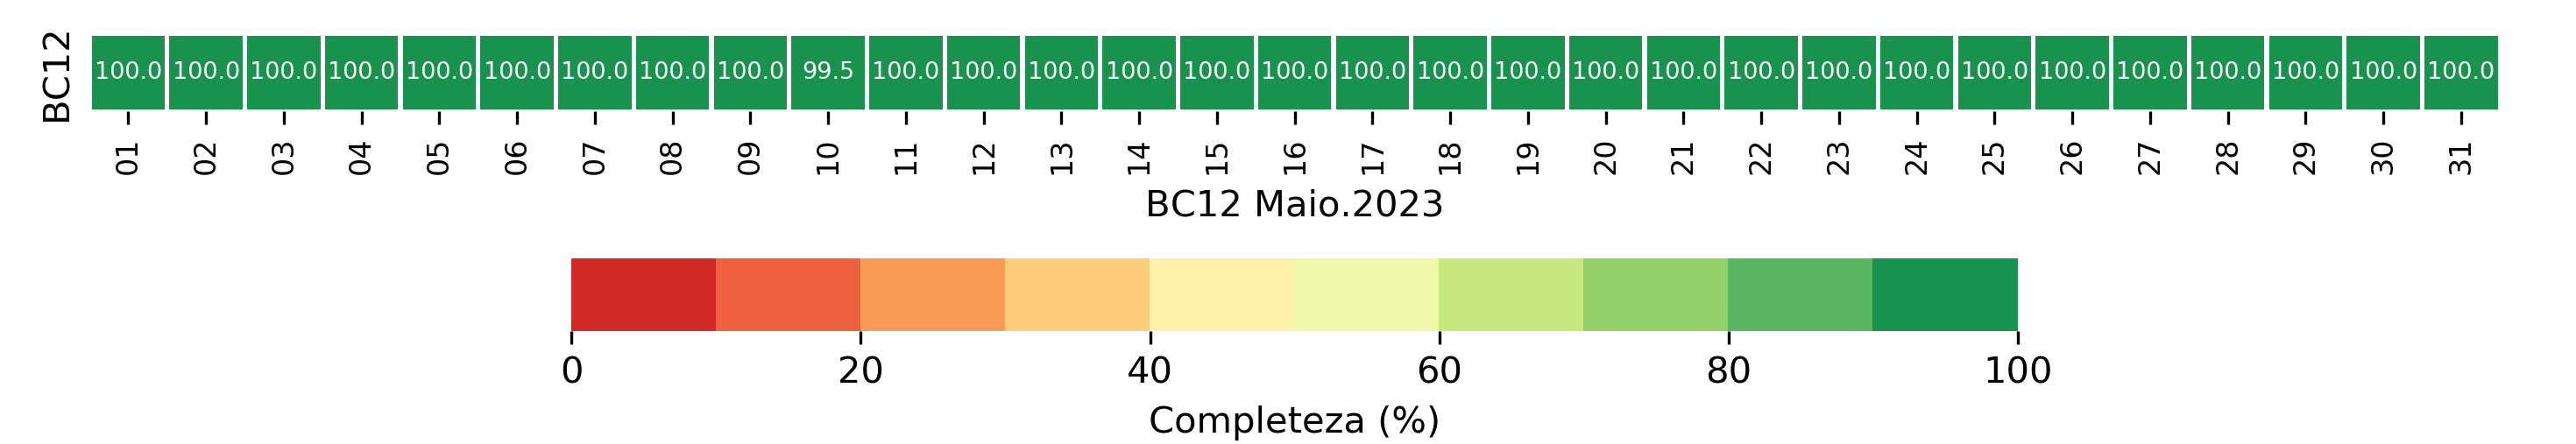
\includegraphics[width=1.0\textwidth]{./boletim/baesa/figuras/bc12_completude.png}
    \end{mdframed}
    \caption*{Fonte: IPT}
\end{figure}


\clearpage
\vspace*{\fill}
\begin{center}
    \section*{ANEXO B}
\end{center}
\vspace*{\fill}
\clearpage
\newpage

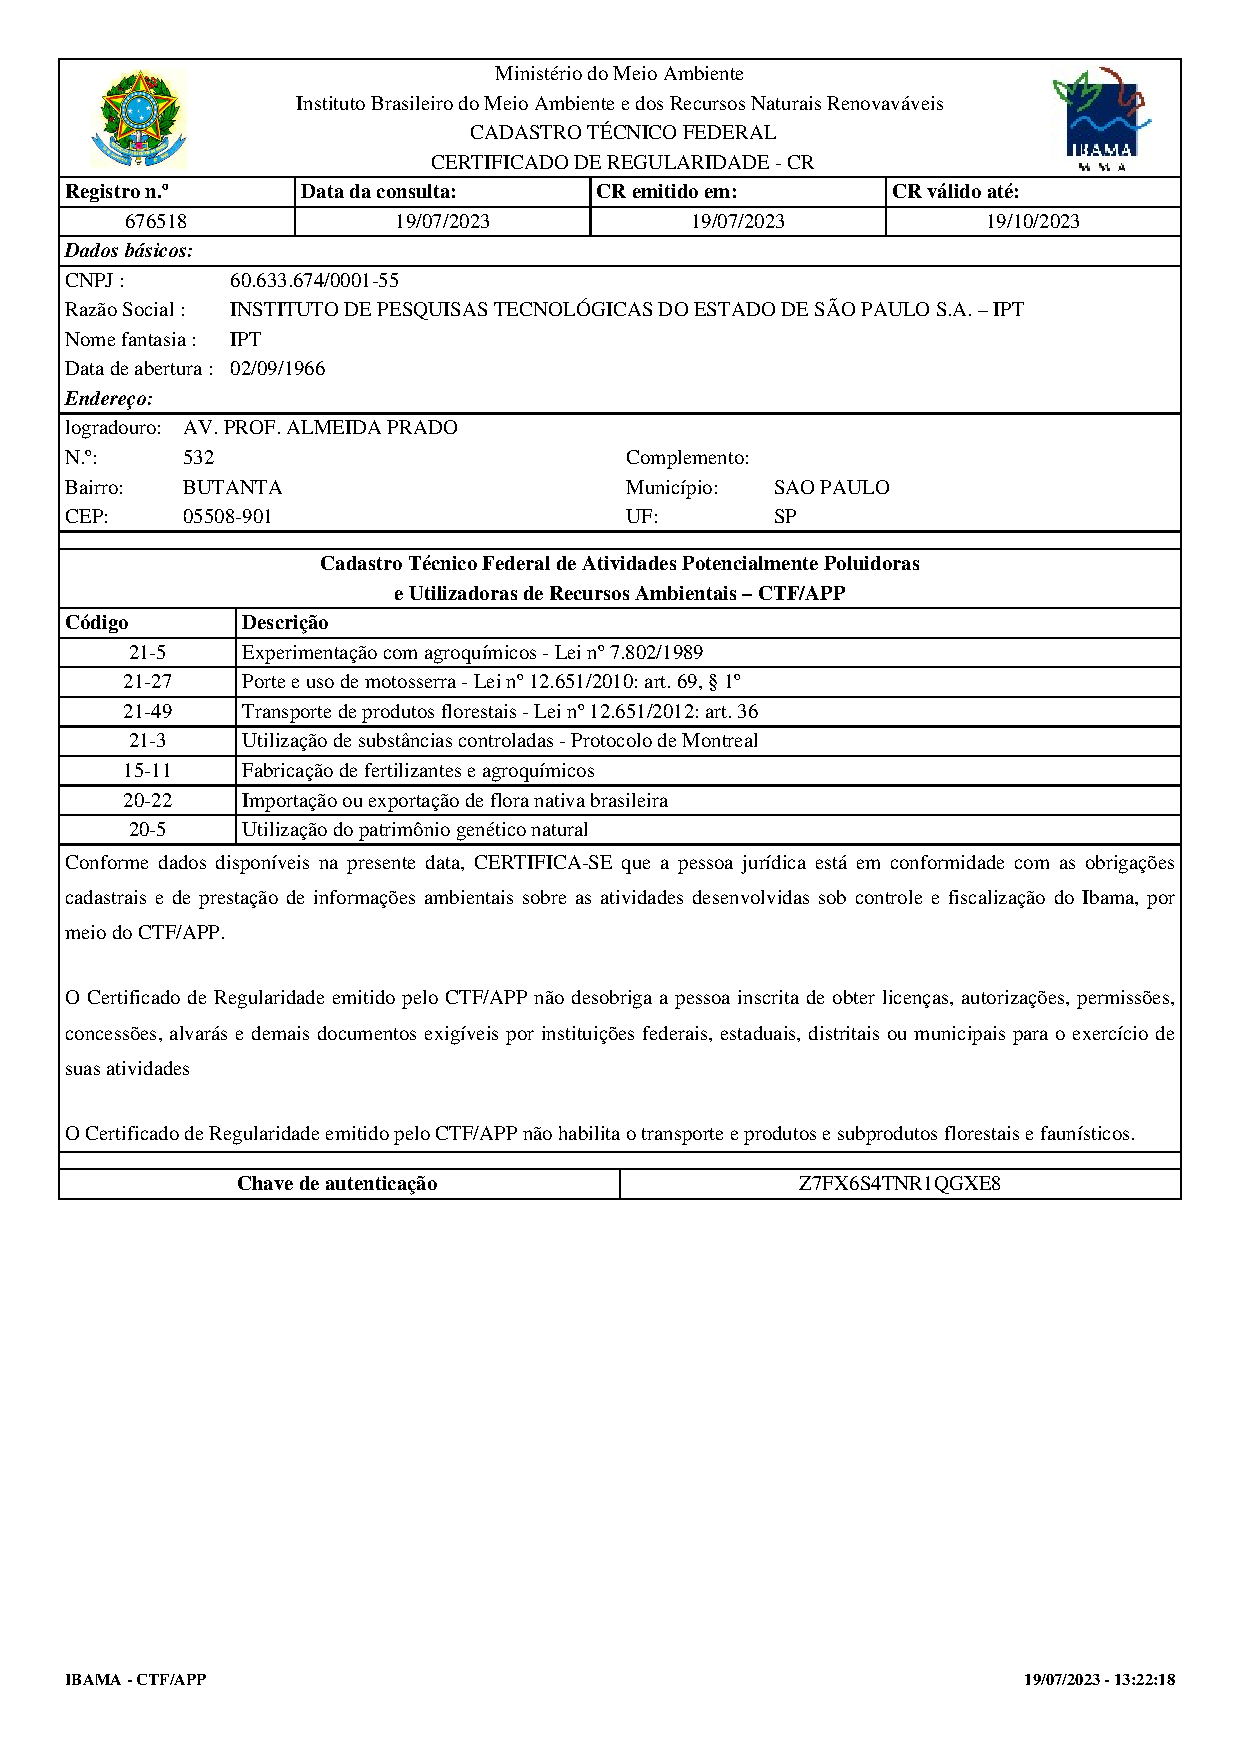
\includepdf[pages=1,scale=0.8,pagecommand{}]{../boletim/baesa/docs/cr_ibama.pdf}
\clearpage
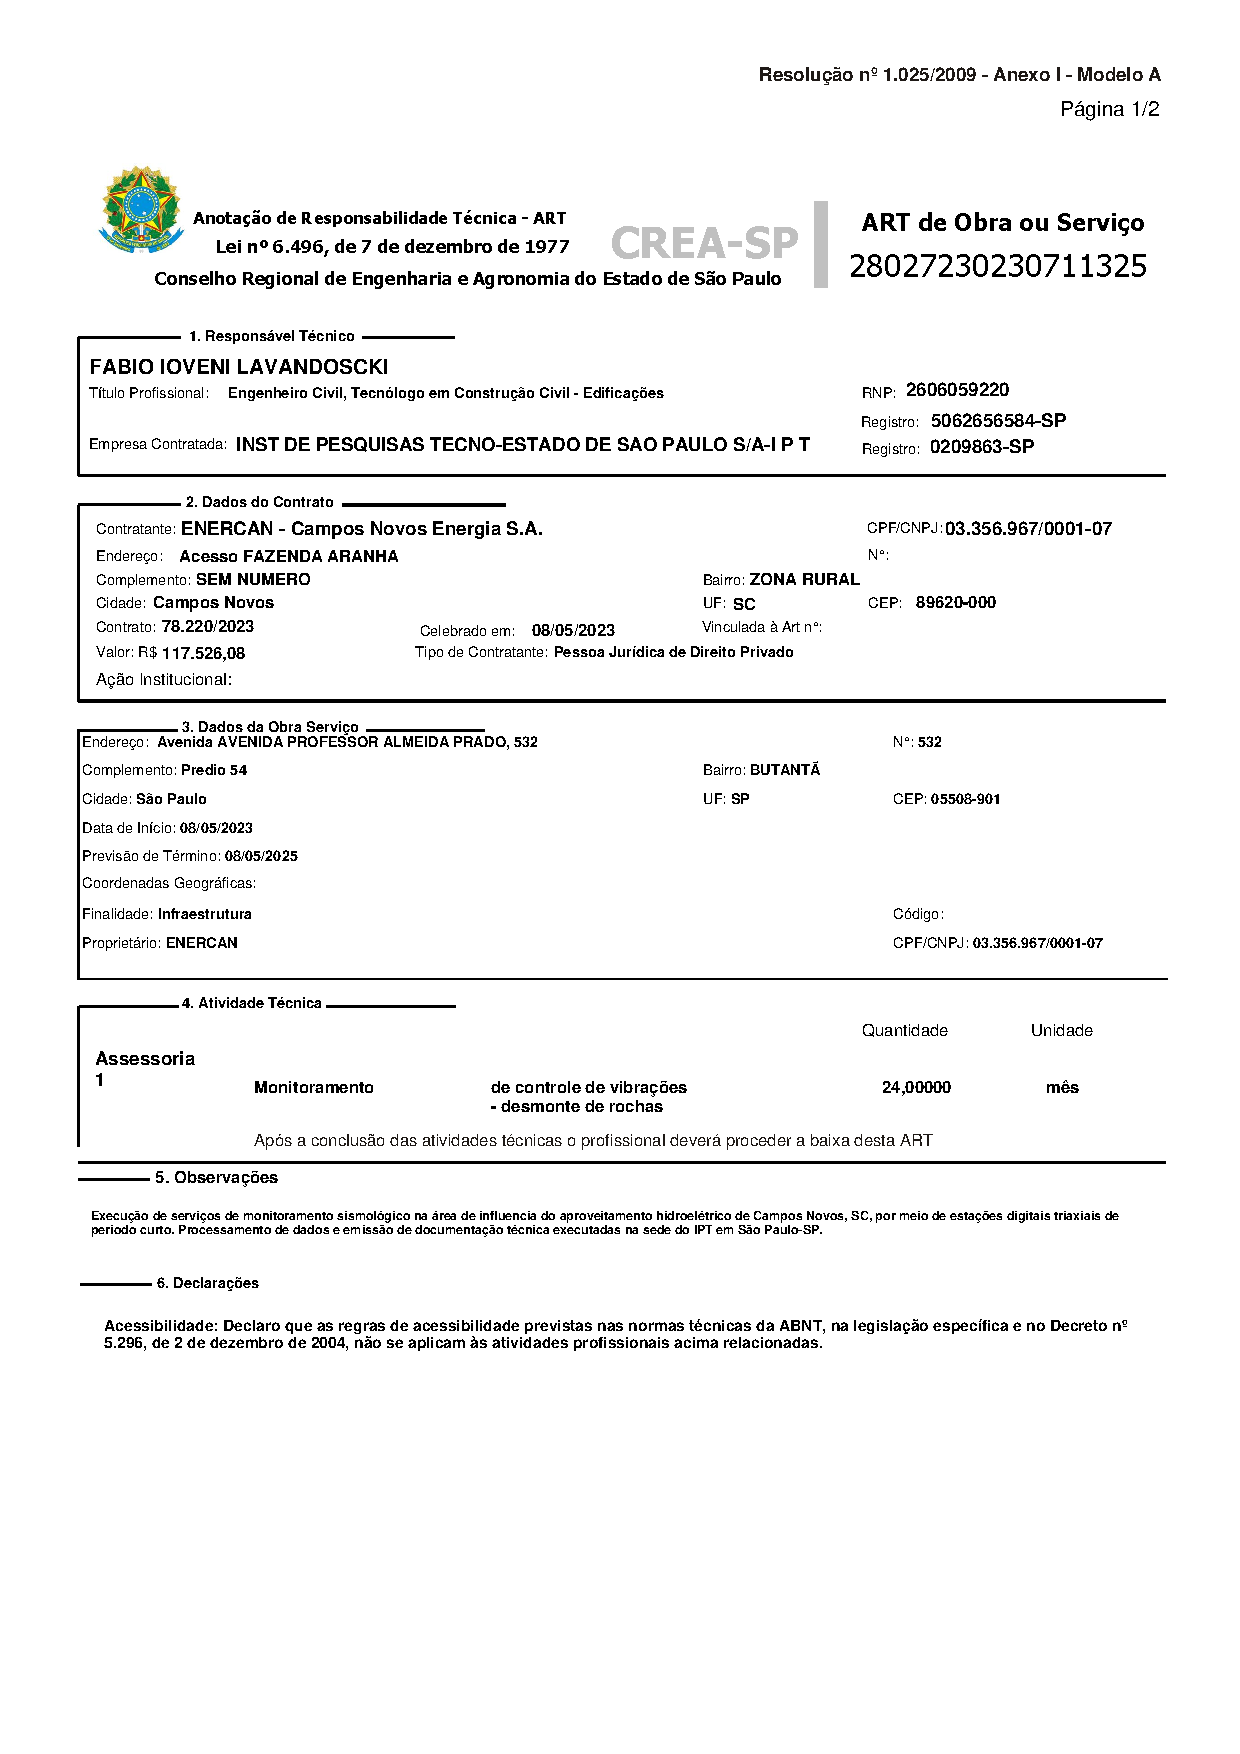
\includepdf[pages=1-2,scale=0.8,pagecommand{}]{../boletim/baesa/docs/ART_Enercan_Ass.pdf}
\clearpage
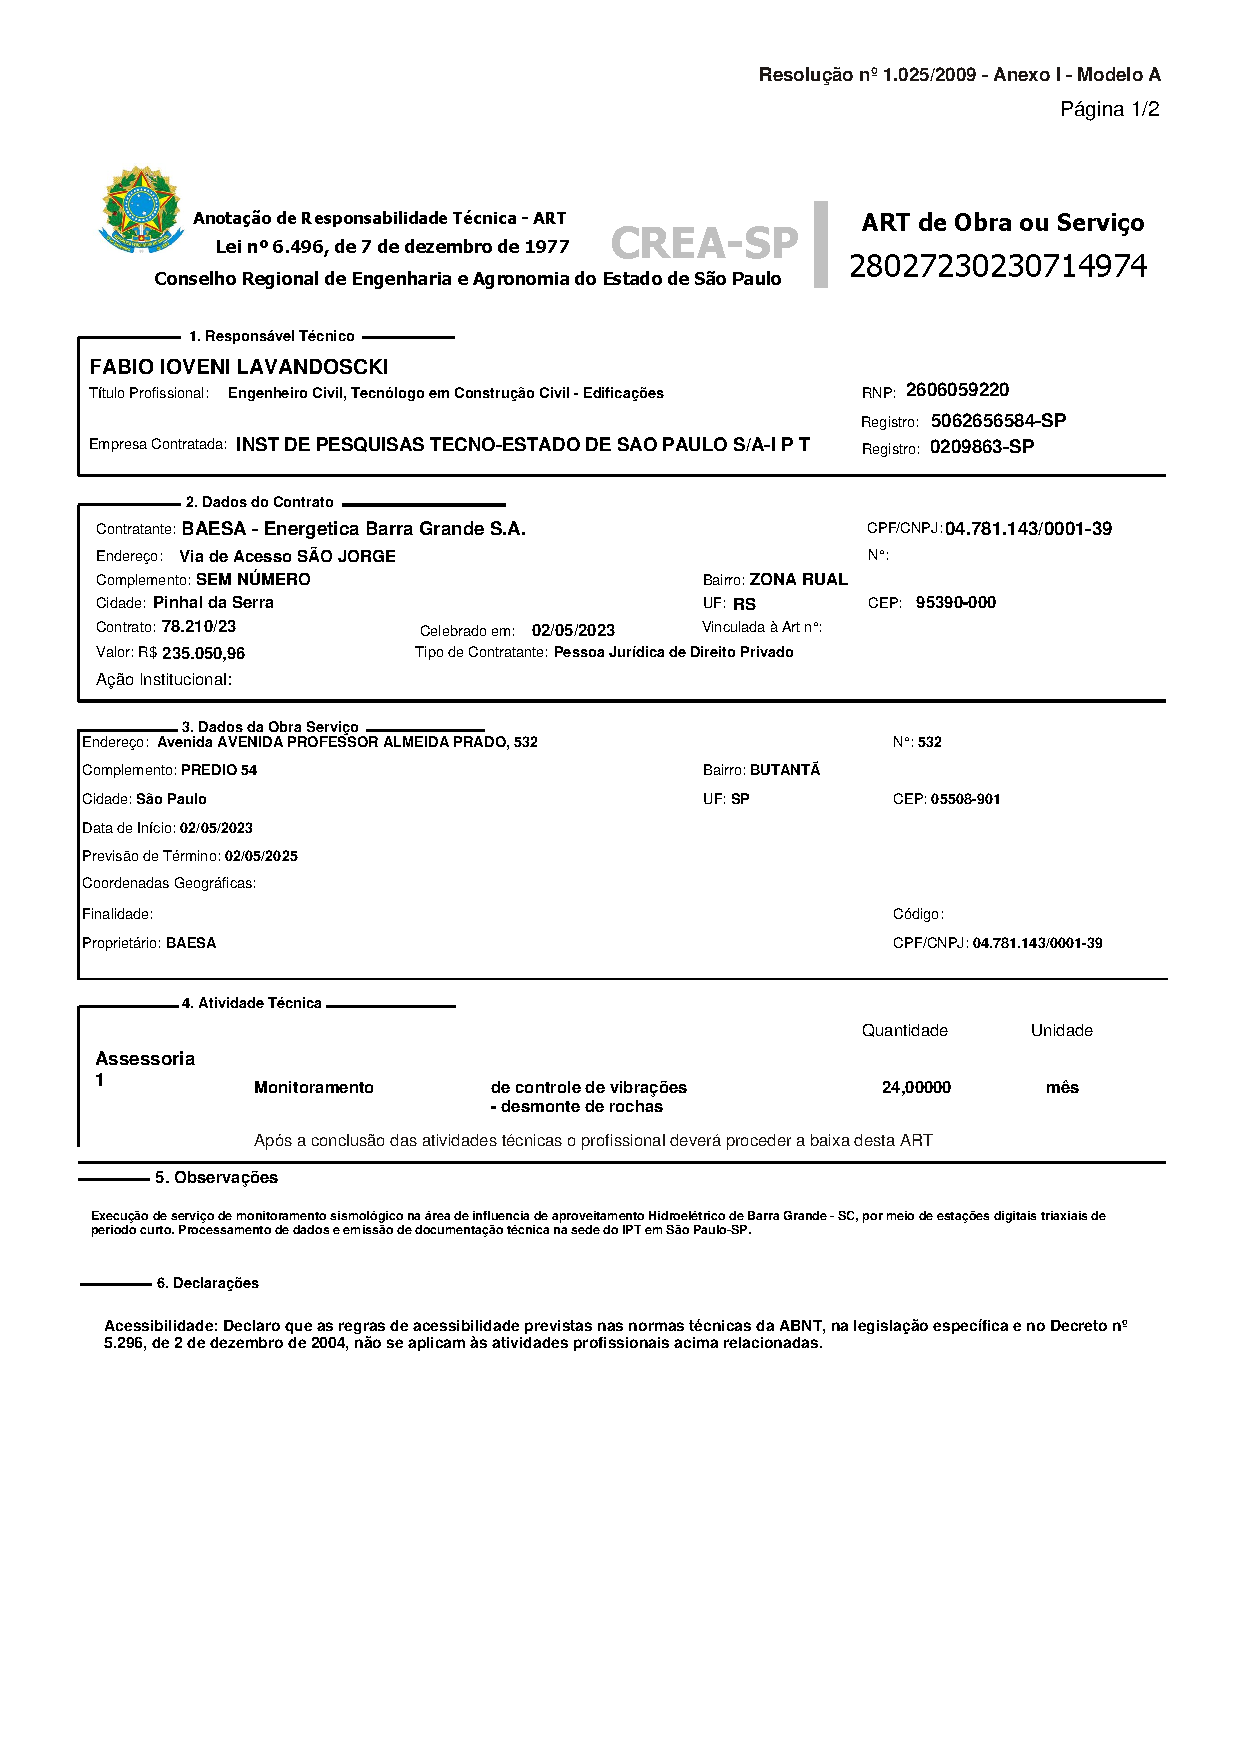
\includepdf[pages=1-2,scale=0.8,pagecommand{}]{../boletim/baesa/docs/ART_Baesa_Ass.pdf}




\clearpage
\newpage

% Bibliografia
\section{REFERÊNCIAS BIBLIOGRÁFICAS}
C. F. RICHTER, \textit{Elementary Seismology}, W. H. Freeman and Co., San Francisco, 1958, 768 pp.
%\renewcommand{\refname}{REFERÊNCIAS}
%\addcontentsline{toc}{section}{REFERÊNCIAS}
%\bibliography{ref}


\end{document}
